\section{Unsupervised Adversarial Invariance}
\label{sec:uaif}

% Predicting target variables ($y$) from data ($x$) involves learning associations between $y$ and the underlying factors of variation of $x$ from data. This is often modeled as the estimation of the conditional probability $p(y|x)$ from available training data. However, $x$ often contains nuisance factors ($z$) that are unrelated to the task of $y$-prediction and supervised learning algorithms often learn to mistakenly associate some $z$ to $y$.

In this section, we describe a generalized framework for unsupervised induction of invariance to nuisance factors by disentangling information required for predicting $y$ from other unrelated information contained in $x$ through the incorporation of data reconstruction as a competing task for the primary prediction task and a disentanglement term in the training objective. This is achieved by learning a split representation of data as $e = [e_1 \ e_2]$, such that information essential for the prediction task is pulled into $e_1$ while all other information about $x$ migrates to $e_2$. We present an adversarial instantiation of this framework, which we call Unsupervised Adversarial Invariance.

\subsection{Unsupervised Invariance Induction}
\label{sec:uaif_gen}

Data samples ($x$) can be abstractly represented as a set of underlying factors of variation $F = \{f_i\}$. This can be as simple as a collection of numbers denoting the position of a point in space or as complicated as information pertaining to various facial attributes that combine non-trivially to form the image of someone's face. Understanding and modeling the interactions between factors of variation of data is an open problem. However, supervised learning of the mapping of $x$ to target ($y$) involves a relatively simpler (yet challenging) problem of finding those factors of variation ($F_y$) that contain all the information required for predicting $y$ and discarding all the others ($\overline{F}_y$). Thus, $F_y$ and $\overline{F}_y$ form a partition of $F$, where we are more interested in the former than the latter. Since $y$ is independent of $\overline{F}_y$, i.e., $y \perp \overline{F}_y$, we get $p(y|x) = p(y|F_y)$. Estimating $p(y|x)$ as $q(y|F_y)$ from data is beneficial because the nuisance factors, which comprise $\overline{F}_y$, are never presented to the estimator, thus avoiding inaccurate learning of associations between nuisance factors and $y$. This forms the basis for ``feature selection'', a research area that has been well-studied.

We incorporate the idea of splitting $F$ into $F_y$ and $\overline{F}_y$ in our framework in a more relaxed sense as learning a disentangled latent representation of $x$ in the form of $e = [e_1 \ e_2]$, where $e_1$ aims to capture all the information in $F_y$ and $e_2$ that in $\overline{F}_y$. Once trained, the model can be used to infer $e_1$ from $x$ followed by $y$ from $e_1$. More formally, our general framework for unsupervised invariance induction comprises four core modules: (1) an encoder $Enc$ that embeds $x$ into $e = [e_1 \ e_2]$, (2) a predictor $Pred$ that infers $y$ from $e_1$, (3) a noisy-transformer $\psi$ that converts $e_1$ into its noisy version $\tilde{e}_1$, and (4) a decoder $Dec$ that reconstructs $x$ from $\tilde{e}_1$ and $e_2$. Additionally, the training objective contains a loss-term that enforces disentanglement between $Enc(x)_1 = e_1$ and $Enc(x)_2 = e_2$. Figure~\ref{fig:uaif} shows our generalized framework. The training objective for this system can be written as Equation~\ref{eq:uif}.

\vspace{-10pt}
\begin{flalign}
\label{eq:uif}
L = \alpha L_{pred}(y, Pred(e_1)) + \beta L_{dec}(x, Dec(\psi(e_1),e_2)) + \gamma L_{dis}((e_1, e_2)) \ \ \ \ \ \ \ \qquad \qquad \qquad \nonumber \\
= \alpha L_{pred}(y, Pred(Enc(x)_1)) + \beta L_{dec}(x, Dec(\psi(Enc(x)_1), Enc(x)_2)) + \gamma L_{dis}(Enc(x))
\end{flalign}
% \vspace{-10pt}

The predictor and the decoder are designed to enter into a \textit{competition}, where $Pred$ tries to pull information relevant to $y$ into $e_1$ while $Dec$ tries to extract all the information about $x$ into $e_2$. This is made possible by $\psi$, which makes $\tilde{e}_1$ an unreliable source of information for reconstructing $x$. Moreover, a version of this framework without $\psi$ can converge to a degenerate solution where $e_1$ contains all the information about $x$ and $e_2$ contains nothing (noise), because absence of $\psi$ allows $e_1$ to be readily available to $Dec$. The competitive pulling of information into $e_1$ and $e_2$ induces information separation such that $e_1$ tends to contain more information relevant for predicting $y$ and $e_2$ more information irrelevant to the prediction task. However, this competition is not sufficient to completely partition information of $x$ into $e_1$ and $e_2$. Without the disentanglement term ($L_{dis}$) in the objective, $e_1$ and $e_2$ can contain redundant information such that $e_2$ has information relevant to $y$ and, more importantly, $e_1$ contains nuisance factors. The disentanglement term in the training objective encourages the desired clean partition. Thus, \emph{essential} factors required for predicting $y$ concentrate into $e_1$ and all other factors migrate to $e_2$.

% \begin{figure}
% \captionsetup[subfigure]{font=scriptsize,labelfont=scriptsize,aboveskip=1pt,belowskip=1pt}
% \centering
% \begin{subfigure}{0.49\textwidth}
% \centering
% 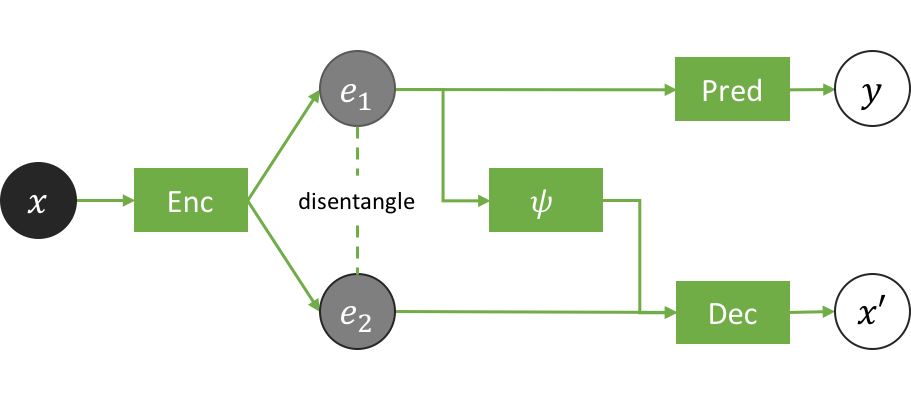
\includegraphics[width=\textwidth]{img/uaif.png}
% \caption{\label{fig:uaif}}
% \end{subfigure}
% \hfill
% \begin{subfigure}{0.49\textwidth}
% \centering
% 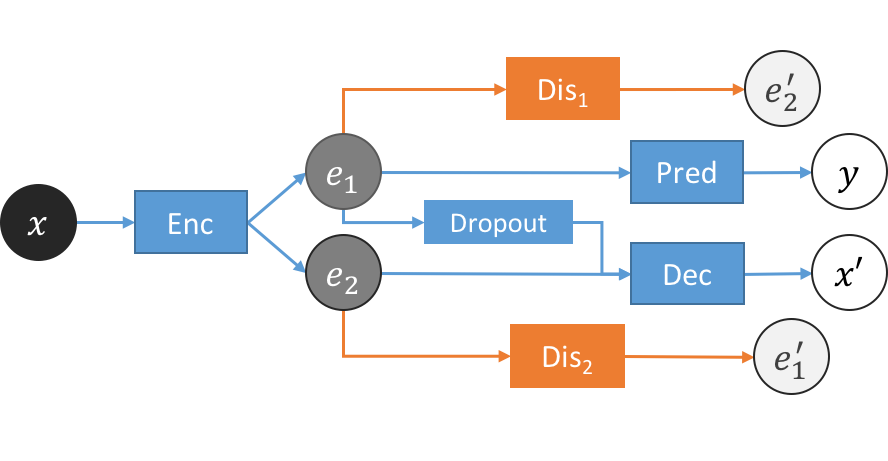
\includegraphics[width=\textwidth]{img/uai.png}
% \caption{\label{fig:uai_md}}
% \end{subfigure}
% \caption{\label{fig:uai}(a) Unsupervised Invariance Induction Framework and (b) Adversarial Model Design}
% \end{figure}

\begin{figure}
\captionsetup[subfigure]{aboveskip=-5pt,belowskip=-4pt}
\centering
\subcaptionbox{\label{fig:uaif}}{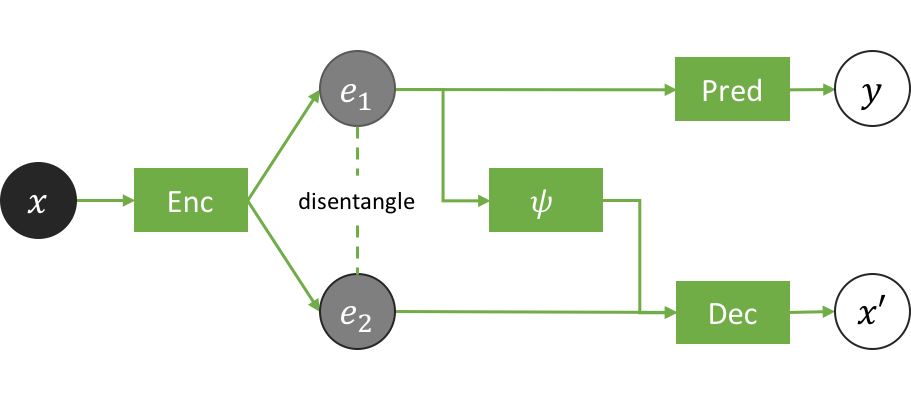
\includegraphics[trim={0 0.3cm 0 0.3cm},clip,width=0.49\textwidth]{img/uaif.png}}
\hfill
\subcaptionbox{\label{fig:uai_md}}{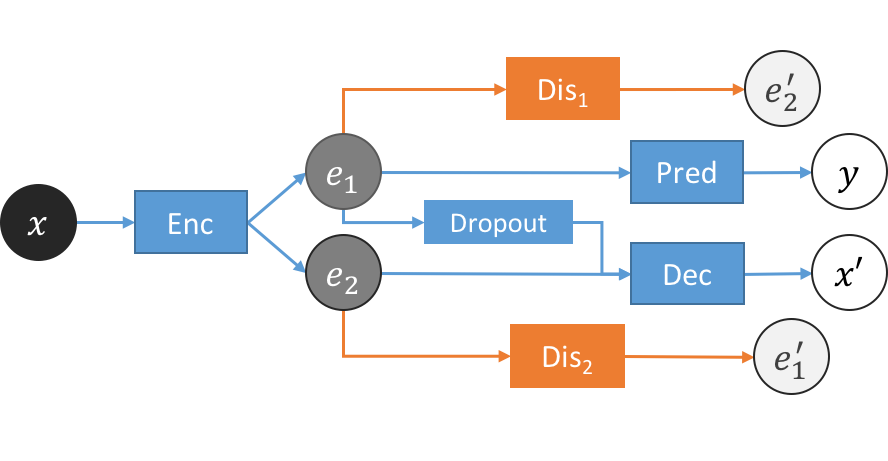
\includegraphics[trim={0 0.3cm 0 0.3cm},clip,width=0.49\textwidth]{img/uai.png}}
\caption{\label{fig:uai}(a) Unsupervised Invariance Induction Framework and (b) Adversarial Model Design}%. $Enc$ encodes $x$ into $e_1$ and $e_2$. $Pred$ uses $e_1$ to predict $y$. $Dec$ uses $\psi(e_1)$ and $e_2$ to reconstruct $x$. $\psi$ is implemented as dropout. Disentanglement is enforced through adversarial modules $Dis_1$ and $Dis_2$.}
\end{figure}

\subsection{Adversarial Model Design and Optimization}
While there are numerous ways to implement the proposed unsupervised invariance induction framework, we adopt an adversarial model design, introducing a novel approach to disentanglement in the process. $Enc$, $Pred$ and $Dec$ are modeled as neural networks. $\psi$ can be modeled as a parametric noisy-channel, where the parameters of $\psi$ can also be learned during training. However, we model $\psi$ as dropout~\cite{bib:dropout} (multiplicative Bernoulli noise) because it provides an easy and straightforward method for noisy-transformation of $e_1$ into $\tilde{e}_1$ without complicating the training process.

We augment these core modules with two adversarial \textit{disentanglers} $Dis_1$ and $Dis_2$. While $Dis_1$ aims to predict $e_2$ from $e_1$, $Dis_2$ aims to do the inverse. Hence, their objectives are in direct opposition to the desired disentanglement, forming the basis for adversarial minimax optimization. Thus, $Enc$, $Pred$ and $Dec$ can be thought of as a composite model ($M_1$) that is pit against another composite model ($M_2$) containing $Dis_1$ and $Dis_2$. Figure~\ref{fig:uai_md} shows our complete model design with $M_1$ represented by the color blue and $M_2$ with orange. The model is trained end-to-end through backpropagation by playing the minimax game described in Equation~\ref{eq:uai}.

\vspace{-10pt}
\begin{align}
\min_{Enc, Pred, Dec} \ \ &\max_{Dis_1, Dis_2} J(Enc, Pred, Dec, Dis_1, Dis_2); \ \ \text{where:} \nonumber \\
% \text{where}\qquad \qquad \qquad & \nonumber \\
J(Enc, Pred, &Dec, Dis_1, Dis_2) \nonumber \\
= \ \alpha L_{pred} \bigl(y, &Pred(e_1) \bigr) + \beta L_{dec} \bigl(x, Dec(\psi(e_1), e_2)\bigr) + \gamma \tilde{L}_{dis} \bigl((e_1, e_2) \bigr) \nonumber \\
= \ \alpha L_{pred} \bigl(y, &Pred(Enc(x)_1) \bigr) + \beta L_{dec} \bigl(x, Dec(\psi(Enc(x)_1)), Enc(x)_2))\bigr) \nonumber \\
+ \ \gamma &\bigl\{\tilde{L}_{dis_1} \bigl(Enc(x)_2, Dis_1(Enc(x)_1)\bigr) + \tilde{L}_{dis_2} \bigl(Enc(x)_1, Dis_2(Enc(x)_2)\bigr)\bigr\}
\label{eq:uai}
\end{align}
% \vspace{-20pt}

We use mean squared error for the disentanglement losses $\tilde{L}_{dis_1}$ and $\tilde{L}_{dis_2}$. We optimize the proposed adversarial model using a scheduled update scheme where we freeze the weights of a composite player model ($M_1$ or $M_2$) when we update the weights of the other. $M_2$ should ideally be trained to convergence before updating $M_1$ in each training epoch to backpropagate accurate and stable disentanglement-inducing gradients to $Enc$. However, this is not scalable in practice. We update $M_1$ and $M_2$ in the frequency ratio of $1:k$. We found $k = 5$ to perform well in our experiments.

